\documentclass[11pt,a4paper,final]{paper}
\usepackage[utf8]{inputenc}
\usepackage{amsmath}
\usepackage{amsfonts}
\usepackage{amssymb}
\usepackage{makeidx}
\usepackage{graphicx}
\usepackage{lmodern}
\usepackage{url}
\usepackage{xfrac}
\usepackage{caption}
\usepackage{subcaption}

\author{Leonardo Alchieri \& Giulia Boschi}

\title{Statistical analysis of covid-19 deaths}
\date{\today}
\bibliographystyle{abbrv}

\begin{document}

\begin{titlepage}
\maketitle
\end{titlepage}
\tableofcontents
\clearpage

\section{Introduction}\label{sec:intro}

This year 2020 will be remembered in the history books as one marked by the \textbf{covid-19} pandemic: as of the time of writing this article, more than 3 million people have been infected worldwide, with almost $250$ thousands declared dead because of it.  Indeed, we, humanity as a whole, are experiencing one of the greatest challenges of our generation, and the response and effectiveness of governments around the world will weight on how many people will perish in this pandemic. As for Italy, which shall be the focus of our analysis, both for geographical purposes (at the time of writing, we are located in northern Italy) and for impact on the population, data from the \textit{Istituto Superiore di Sanità} shows how most of the deceased people are in the older spectrum of the population: the average age of death due to SARS-CoV-2 pneumonia is 81 years old. \cite{remuzzi2020covid} 

While most of the data regarding deaths is the most accurate health workers and facilities manage to garner in such dreadful instances, one might argue its absolute correctness. Indeed, one can expect that, especially in the early days of the pandemic in a specific location, some covid-19 related deceased might go unnoticed, e.g. due to lack of tests in the population or overcapacity in health care facilities. In our work, we decided to focus on estimating, as accurately as possible, both the impact of covid-19 on ``standard" yearly deaths in the first quarter of the year and the disparity with official death data. 

We shall first describe in detail the data used to carry out this analysis, especially its relevant limitations. Then we will show a statistical model aimed at forecasting covid-less deaths in the first quarter of 2020; and, finally, we will describe our results when such model is applied and the comparison with official deceased data. In the end, we will draw up some conclusions and limitations of our work.

\section{Dataset description}\label{sec:descr}
%Analyzed data were made available by \textbf{ISTAT } (\textit{National Institute of Statistics}) and contain information about deaths distinguished by women, men and total, town and day, and the data are referred to the period from 1st January to 20th April from 2015 to 2020.
The main dataset we employed was made available by \textbf{ISTAT} recently and it contains information about reported deaths in Italy for the first 4 months of 2015-2020. In particular, it contains, in its attributes, information about the number of deceased per: day, municipality and sex; each municipality has also specified information regarding its administrative location, i.e. province and region. 
\footnote{https://www.istat.it/it/archivio/240401} 

In our work, we decided to aggregate data at Regional level, i.e. focus only on Lombardy in particular, for lack of data regarding official deceased locally; we also opted to eliminate, in a preliminary cleaning, any data marked as ``unavailable" in 2020. In these latter cases, we decided it was best just to eliminate them, due to the small amount of such missing values; if one carries out a similar analysis, he or she might want, in some cases, to substitute them with averages taken from previous years.
In Figure \ref{fig:lomb_death_2015_2020}, one can clearly see a very sharp increase in deaths in Lombardy starting from March 2020: this is in line with the arrival of the pandemic in Northern Italy. In particular, even at first glance from this representation, one can see the striking effect of the virus. We will show and discuss this effect in more detail later.

\begin{figure}[h]
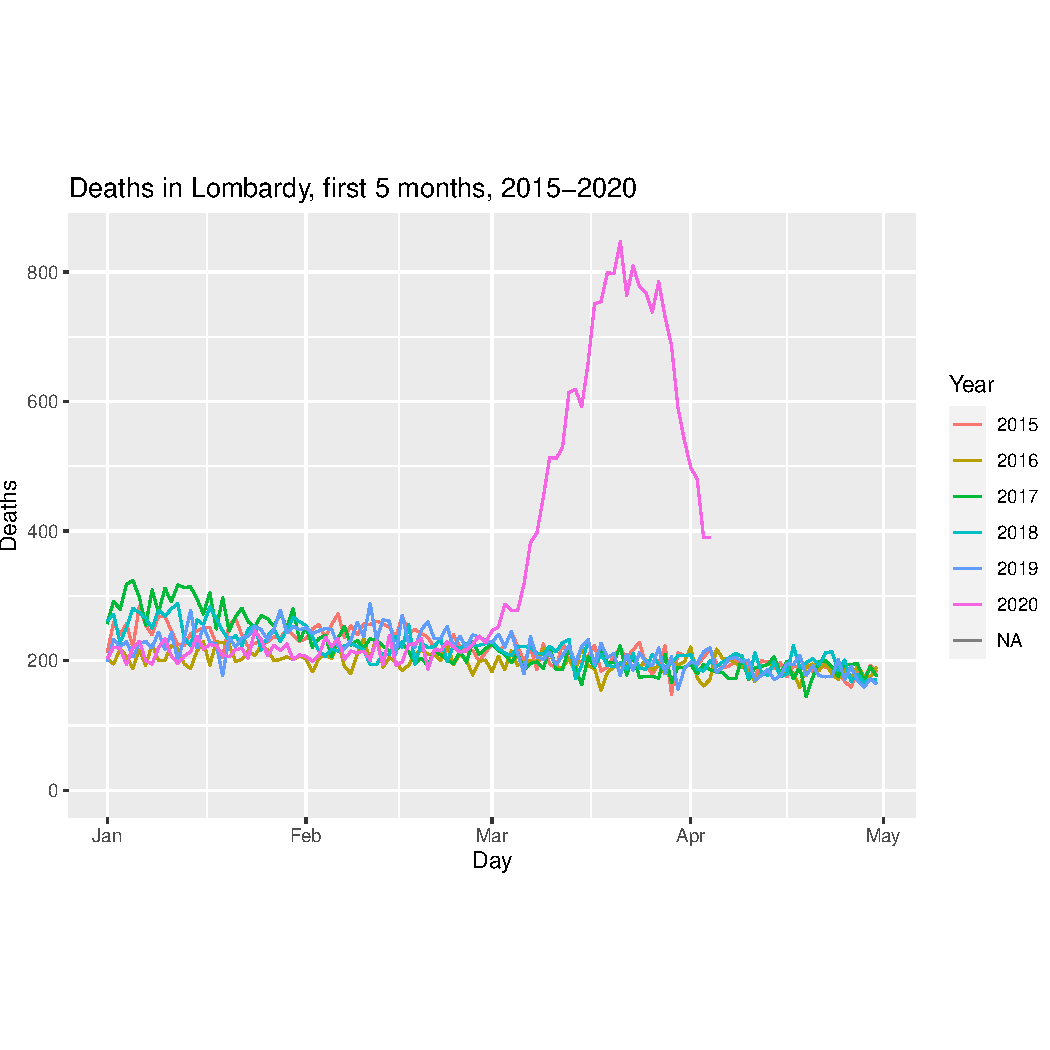
\includegraphics[width=\textwidth]{../images/lombardy_deaths_2015_2020.pdf}
\caption{Number of daily deceased in all of Lombardy in the first 5 months of different years.}
\label{fig:lomb_death_2015_2020}
\end{figure}
%/The analysis were carried out on aggregated data at regional level, excluding municipalities whose data were not available for 2020 (‘DECESSI’ = 9999). 

Between the many attributes present in the dataset, the one named \texttt{DATA\_INIZIO\_DIFF} puzzled us: the interpretation we have given is that of \textit{beginning date of sharing data from the municipalities} to \textbf{ISTAT}. Analyzing in detail this attribute, we discovered that each municipality had only one such value, thus they were disjointed in it; for such, we did not need to operate any cleaning/integration, and thus we could keep all of those who contained this attribute, i.e. who were not marked as \textit{not available} (\texttt{Data 2020 n.a.}). 

From what we have described, we managed to garner data about 622 municipalities in the administrative region of Lombardy (Figure \ref{fig:comuni_dati}).\footnote{Interactive version: \protect\url{https://public.tableau.com/profile/giulia.boschi#!/vizhome/comuni_disponibili/Dashboard1}} In particular, according to the official documentation of \textbf{ISTAT}, this data was taken from those cities and towns whose deaths rate in 2020 was 20\% higher than average. As such, one might argue, they represent only those places were the SARS-CoV-2 virus afflicted noticeable deaths, compared to not having it. We decided to work with this assumption, as it gave us a more effective approach; we will also show, in the results, how it is not far fetched and consistent with what one might expect. 

\begin{figure}[h]
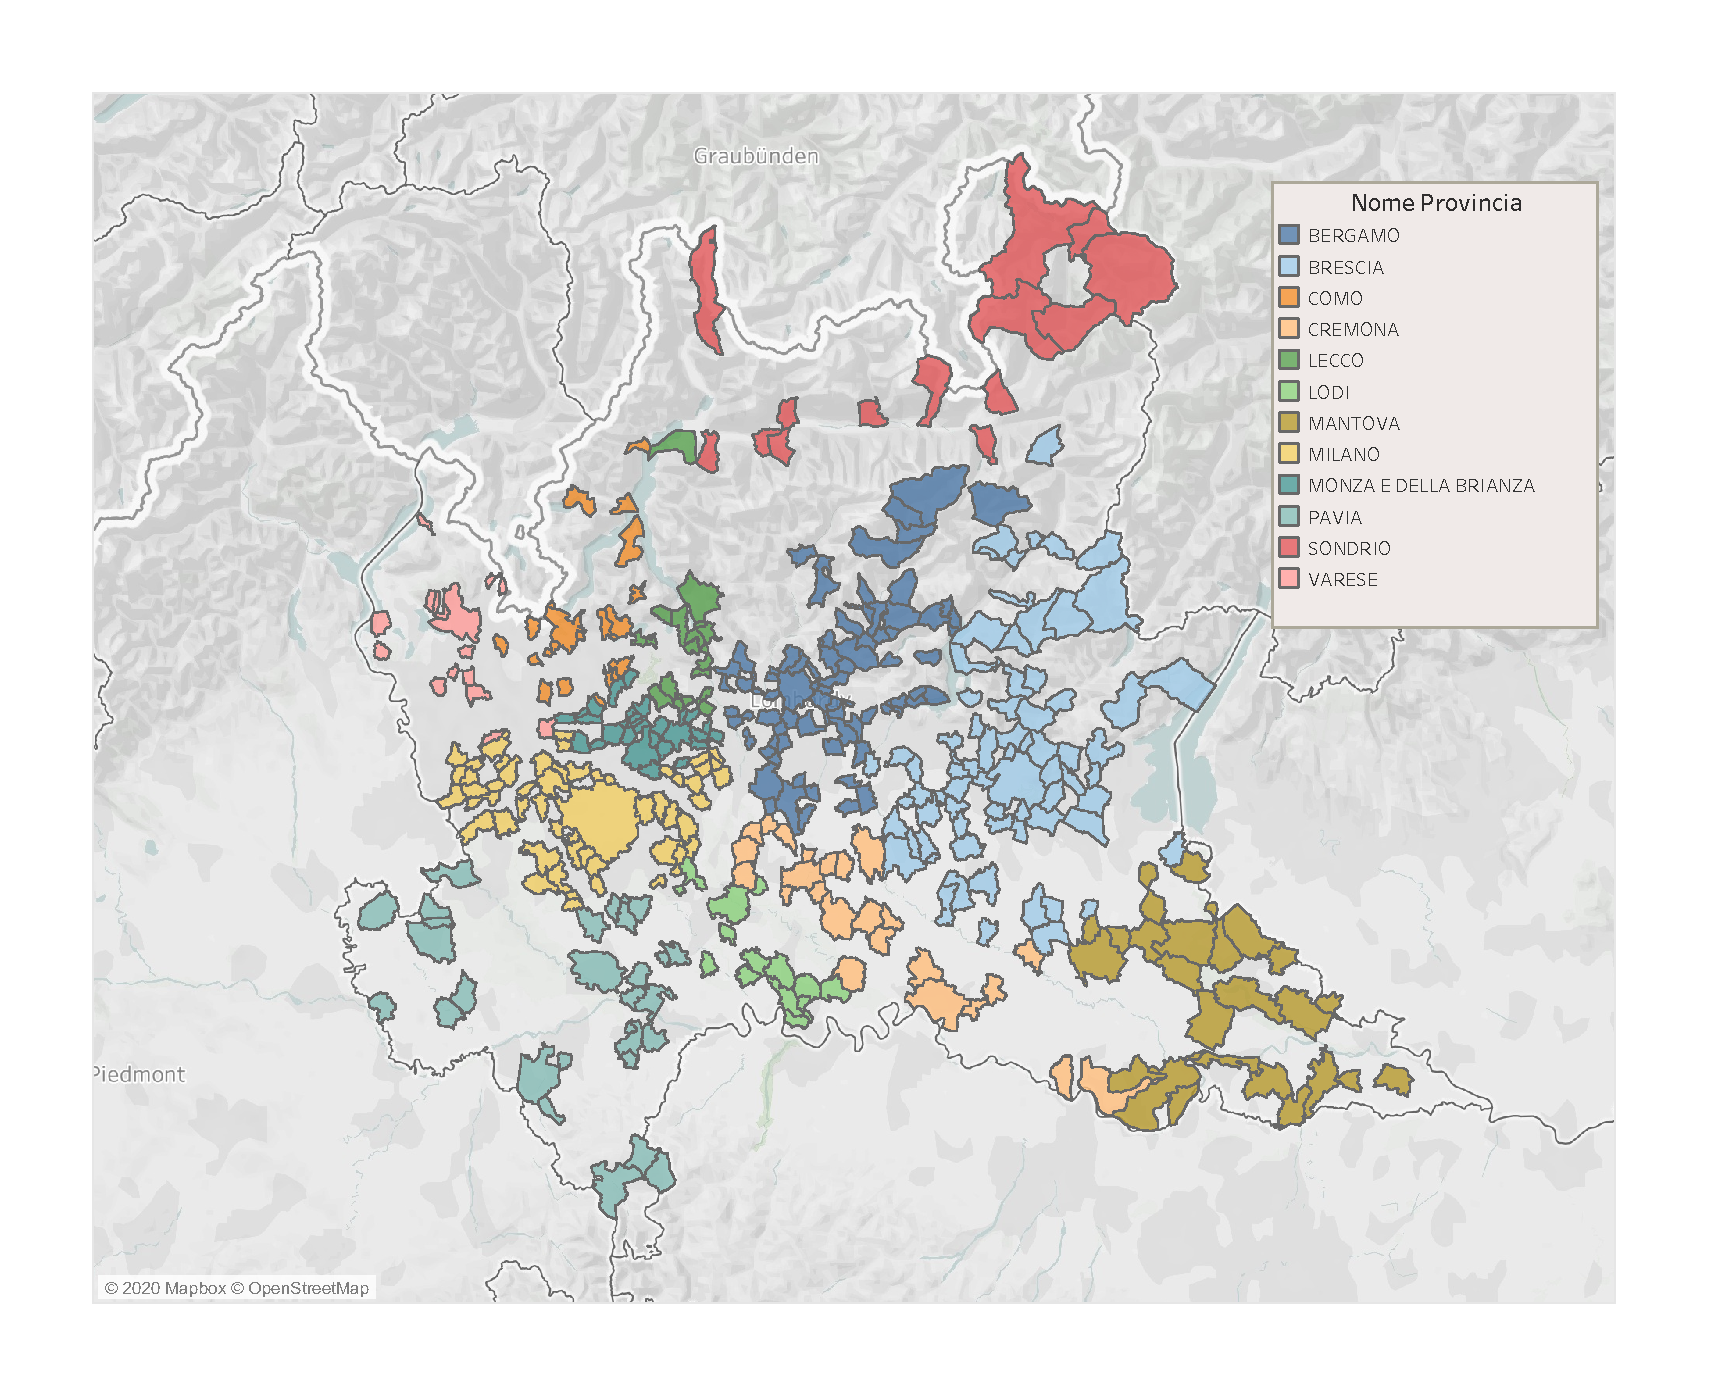
\includegraphics[width=\textwidth]{../images/lombardy_municipalities.pdf}
\caption{Available municipalities in Lombardy. 
Data source: \protect\url{http://www.geoportale.regione.lombardia.it/}.}
\label{fig:comuni_dati}
\end{figure}

From what we have just described, we took as hypothesis in our work that the municipalities at hand, and only those, contained all of the covid-19 deceased in Lombardy. Let's call the total number of death in 2020 in Lombardy as $M_{tot}$ for simplicity; we can infer that it may be composed of two parts, one given by the deaths caused, directly or indirectly, by the \textit{covid-19} pandemic, $C$, and one for those not caused by it, which we can call, for simplicity, ``standard" $N$. We can assume that all of these components are the sum of municipal components, i.e. the sum of local deaths:
\[
	M_{tot} = \sum_i m_i = C + N = \sum_i c_i + \sum_i n_i
\]
where $m_i$ indicates the number of ceased in the $i$-th municipality. We then shall call with $j$ those municipalities that have had covid-19 deaths, and with $k$ those who lack them. As such, with our hypothesis, the $j$ municipalities are those we have information about in 2020. We can write:
\[
	M_{tot} = \sum_j n_j + \sum_k n_k + \sum_j c_j 
\]
where $N = \sum_j n_j + \sum_k n_k $ and $C = \sum_j c_j $. 

We demonstrate briefly how, even with missing information regarding the $k$ municipalities, we are able to estimate $C$. Indeed, if we do not have $k$, we can only have a partial total:
\[
	M^\prime_{quasi-tot} = \sum_j n_j + \sum_j c_j 
\]
In order to estimate $C$, we can create a model, e.g. based on previous years data, that would estimate $\sum_j n_j$; we shall call this estimator $\hat N^\prime$. Thus, in order to estimate $C$ have can easily do:
\[
	\hat C = M^\prime_{quasi-tot} - \hat N^ \prime
\]	
and thus, we do not need information regarding those municipalities where covid-19 didn't have an impact. 

Obviously, such argument can be present as merely an hypothesis, which we can not certainly verify. Unfortunately, this is the data at hand and, in such a tumultuous time, it's better than nothing; still, a more accurate future analysis might have all of the municipalities at hand and might allow to discard this restrictive hypothesis.  

In order to draw comparisons, we also took data from the Department of Civil Protection for the Lombardy region regarding official covid-19 deaths. We obviously, as we have said, expect this data to contain an underestimated count.\footnote{\url{httppc/COVID-19/blob/master/dati-regioni/dpc-covid19-ita-regioni.csv}}


\section{Modelling}\label{sec:mod}

In order to distinguish covid-19 related deaths in 2020, as described mathematically in Section \ref{sec:descr}, we needed to create a statistical model. We decided to use the information contained in the previous years' data to achieve this. We show in Figure \ref{fig:lomb_death_2015_2019} the data we used as estimate: as can be seen, all of these years have a very similar trend and comparable number of deaths. At first glance, a few information can be extrapolated, such as the fact that the first few months tend to have a slightly higher number of deaths than the last ones; and that in January 2017 there is a slightly higher number of daily deceased, caused by a bad flu season. \footnote{\url{https://www.repubblica.it/salute/2017/03/18/news/l_anno_nero_dell_influenza_morti_ventimila_anziani_in_piu_-160814115/ }}

\begin{figure}[h]
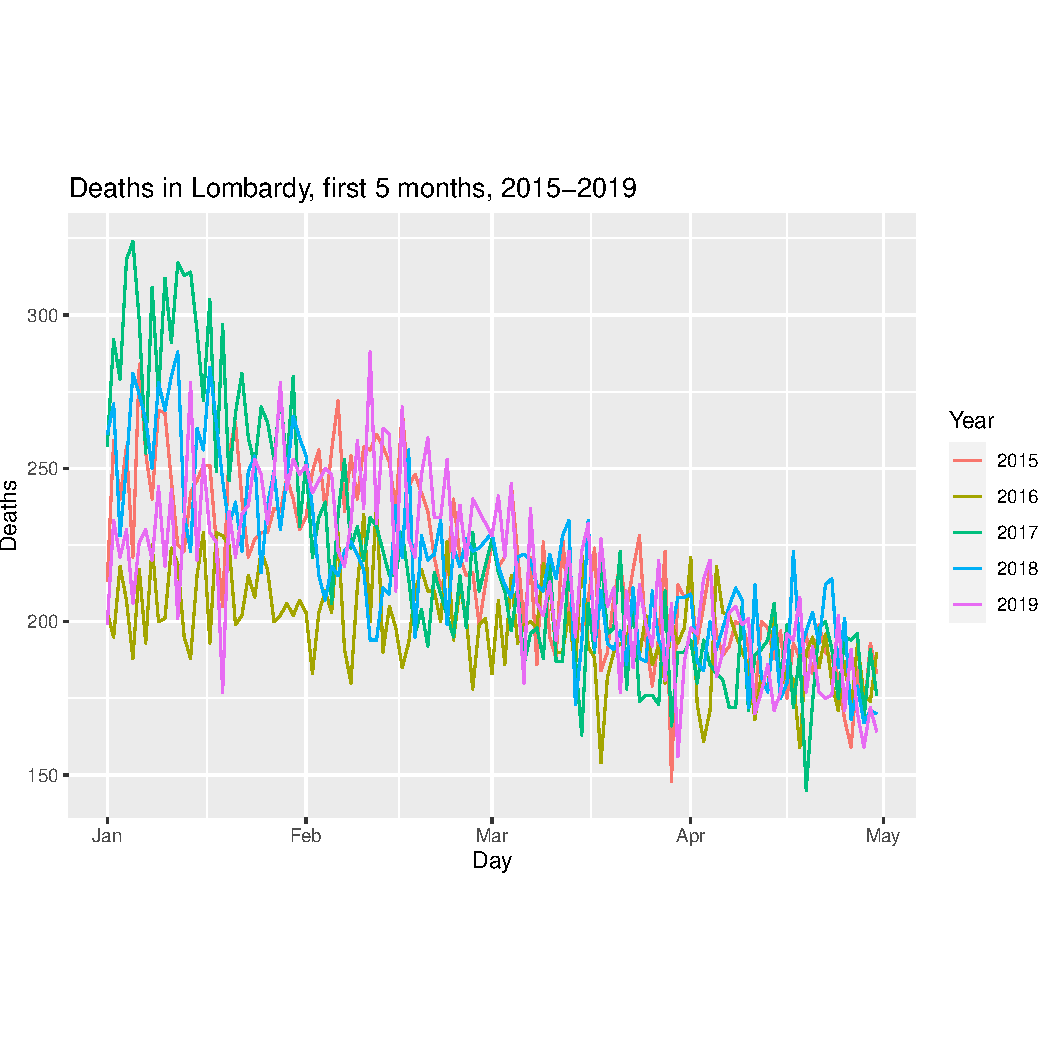
\includegraphics[width=\textwidth]{../images/lombardy_deaths_2015_2019.pdf}
\caption{Number of daily deceased for the first 5 month, for the years 2015-2019.}
\label{fig:lomb_death_2015_2019}
\end{figure}

We decided to aggregate this data as a \textit{time series}, ignoring the missing months of the year for the prediction: while not a very realistic or accurate method, for it ignores a large portion of the year, we believe it can still manage to give a somewhat accurate prediction. Unfortunately, we did not manage to garner daily deaths data for the other months, so we opted for this ``stitching" approach. As alternatives, one could treat the missing months as \textit{missing values} and apply known strategies.\cite{missing_values}

Given the data as a time series, several trends can be usually identifies:\cite{analisi_statistica}
\begin{itemize}
	\item a component indicating medium to long trend, which can be called $T_t$;
	\item a cyclical component $C_t$ that represents succession phases of prosperity and depression, usually included in the trend component, therefore named cycle-trend;
	\item a seasonal component $S_t$ representing the seasonal interim fluctuations;
	\item a stochastic component $a_t$ that is irregular and with an unobservable behavior, present in each historical series.
\end{itemize}
Due to our decision to treat the time series as being connected, i.e. omitting the presence of the other months of the year, the identification of the aforementioned components might be skewed and not truly represent yearly trends. 
We thought the best class of models for our data might be \textbf{ARIMA}, for whose identification we followed the Box and Jenkins procedure:
\begin{enumerate}
	\item identification;
	\item estimation;
	\item diagnostic.
\end{enumerate}
We tried and tested many models, in particular focusing on a few aspects of the timeseries. We report shortly some of these tests:
\begin{itemize}
	\item Due to the higher value of deceased in 2017, as stated previously, we tried to apply a \textbf{model with intervention}, which resulted to be non-significant. \cite{box1975intervention}
	\item The \textit{Box and Cox $\lambda$} was identified to be $0.14$, and thus we did not deploy a logarithmic transformation.
	\item Using the \textit{Dickey Fuller} stationarity test, we found a p-value of $0.09$, which could be accepted significant only with low certainty. Indeed, one might want to apply a differencing operator $\Delta ^d = 1 - B^d$, but we decided not to proceed for it would not make sense to differentiate between April of a year and January of the next. Nevertheless, we believe the time series to be, at worst, almost stationary. 
\end{itemize}
Given these premises, between the many models we tried to evaluate, 2 stood out as best. For all of the models, we used \textit{t test} statistics, $t_i = \frac{\hat \beta_i}{\sigma_{ii}}$, for the estimated parameters; \textit{Jarque-Bera test} for the residual normality, which is based on the fact that a normal distribution has zero skewness and zero kurtosis; and \textit{Ljung Box test}, $Q(K) = n \sum_{k=1}^K w_k p^2(k)$ with $w_k = \sfrac {n+2}{n-k}$, for autocorrelation, in addition to looking at the individual lags.
The models' comparisons were based on the mean absolute percentage error (\textit{MAPE}) and \textit{Akaike’s information criterion }(AIC) indicators. 

The best models we managed to built are the following 2:
\begin{itemize}
	\item $AR(3)$, $(213.9-0.3B-0.3B^2-0.2B^3 ) z_t=a_t$;
	\item $ARMA(3,2)$, $(213.7+0.2B-0.9B^2-0.2B^3 ) z_t=(0.5B-0.5B^2)a_t$.
\end{itemize}
In the second model the values of \textit{AIC} and \textit{MAPE }are slightly lower than the first one; in both models the residuals are not normal for the \textit{Jarque Bera test}, but show a good adaptation in their distribution to a Gaussian curve, as we show in Figure \ref{fig:checkresults}. 

\begin{figure}[h]
	\begin{subfigure}[b]{0.49\textwidth}
		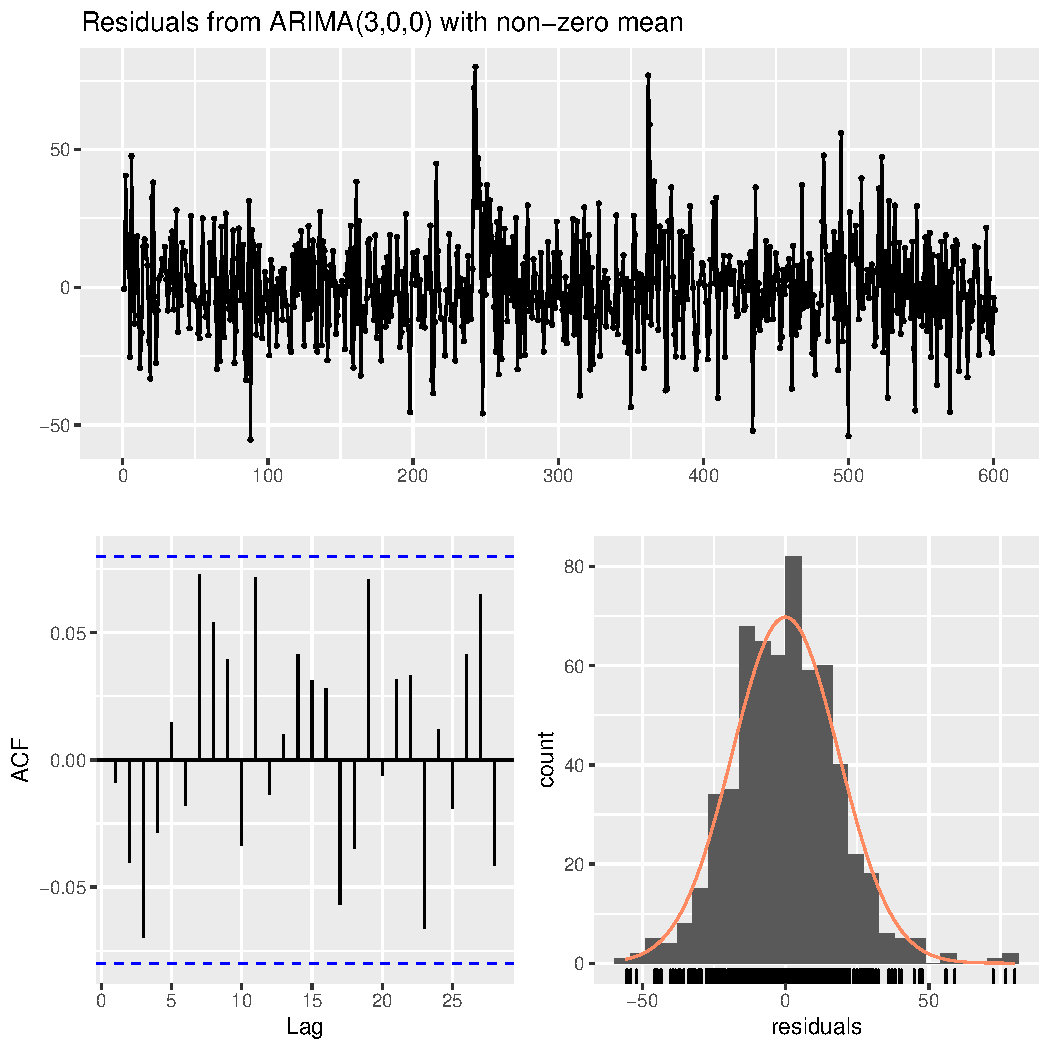
\includegraphics[width=\textwidth]{../images/check_residuals_prime.pdf}
	\end{subfigure}
	\begin{subfigure}[b]{0.49\textwidth}
				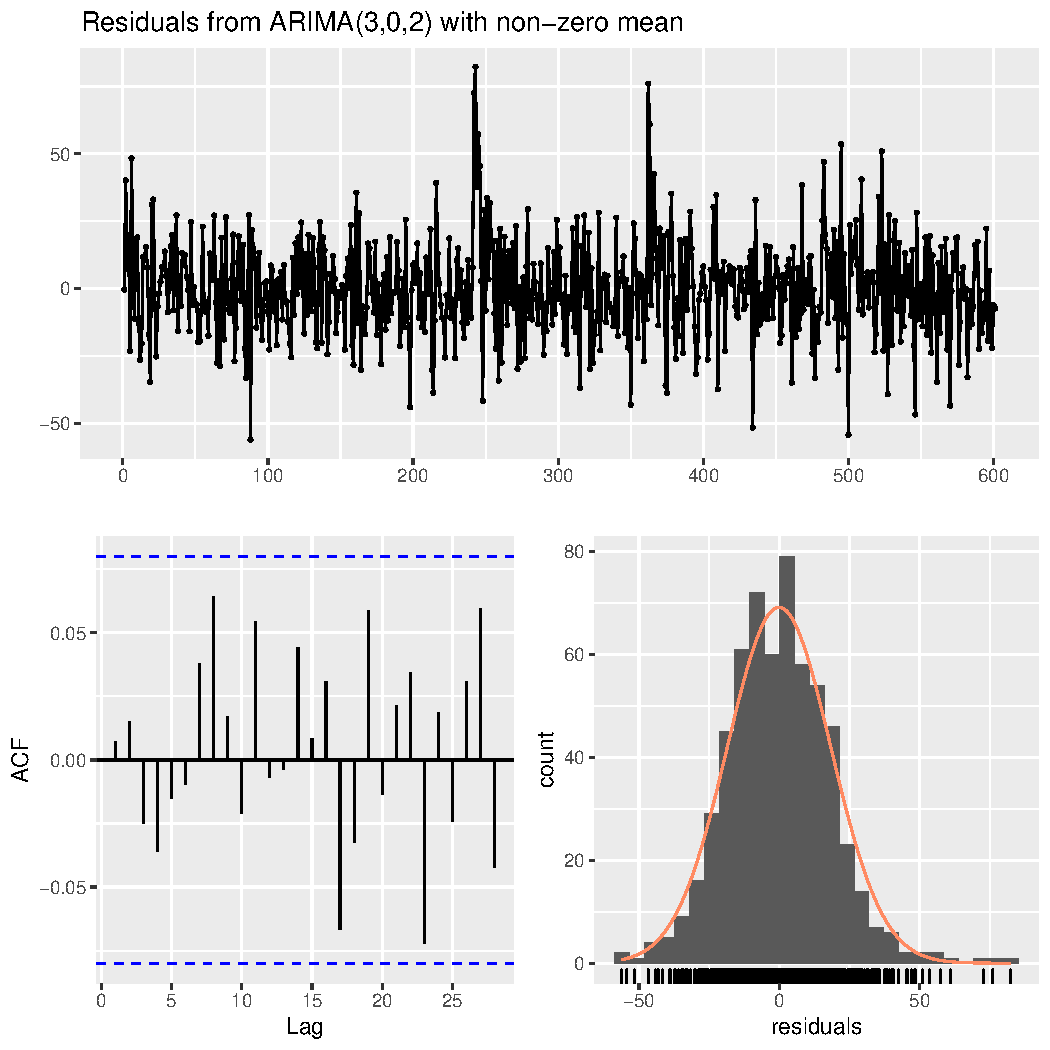
\includegraphics[width=\textwidth]{../images/check_residuals.pdf}	
	\end{subfigure}
	\caption{Output for the \texttt{R} function \texttt{checkresiduals}. On the left, for the $AR(3)$ model, while on the right for the $ARMA(3,2)$.}
	\label{fig:checkresults}
\end{figure}

The second model was chosen because the \textit{Q value }for the \textit{Ljung Box test }is halved, ensuring non correlated error at all meaningfulness thresholds. Regarding both models, and the data at hand, one might argue that a \textit{seasonal} approach could be satisfactory:
it can be shown that there is no significant correlation at any lag level, e.g. over the 5 months available, and thus rendering this techinque not useful.
%we show in Figure \ref{fig:lags} that there is almost no significant correlation at any lag (only 2 out of 120 are slightly significant, i.e. a mere $1\%$, which can be accounted for the fact our confidence interval is at $95\%$).

%\begin{figure}[h]
%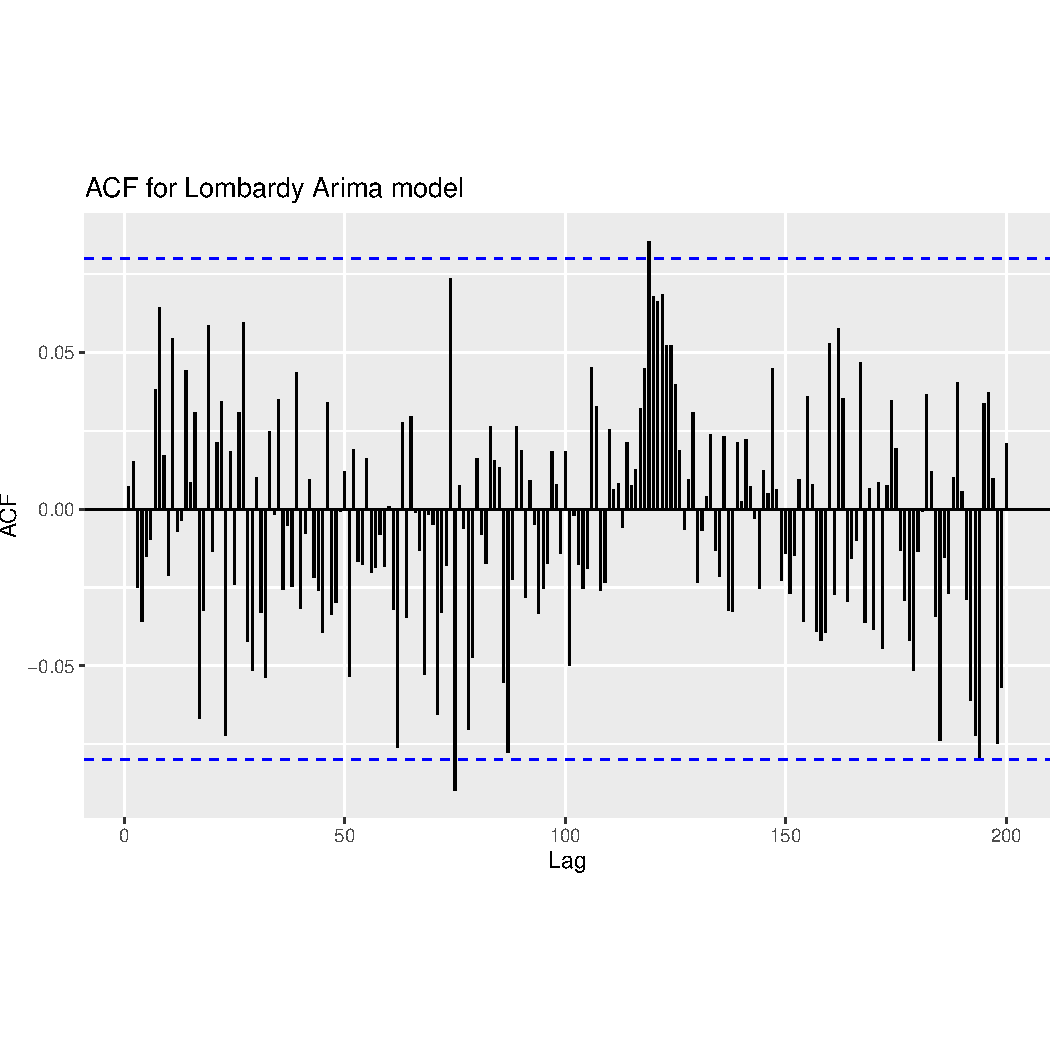
\includegraphics[width=\textwidth]{../images/ACF.pdf}
%\caption{Lags of residuals for the $ARMA(3,2)$ model, with 200 lags, i.e. more than the data for 1 year in our time series.}
%\label{fig:lags} 
%\end{figure}

As an example, we show in Figure \ref{fig:fit_for} the fit of the estimated model over the time series data and an example of future forecast. Indeed, the model is a very good approximation of the given data while the forecast, as one might expect with many points in the future, has quite a large uncertainty. While it tries to render the data decently for the first few days, most of the latter, e.g. from February, are just the average of the time series. 

One might argue that, given such forecast result, which resembles almost entirely the average, that a more straightforward and simple method could be to apply the mean directly. They would indeed be somewhat correct, but we believe that the capacity to predict differently the first few days can have an interesting impact. Nevertheless, our decision to use the model does not hinder us in any way, compared to the simpler approach.

\begin{figure}[h]
	\begin{subfigure}[b]{0.49\textwidth}
	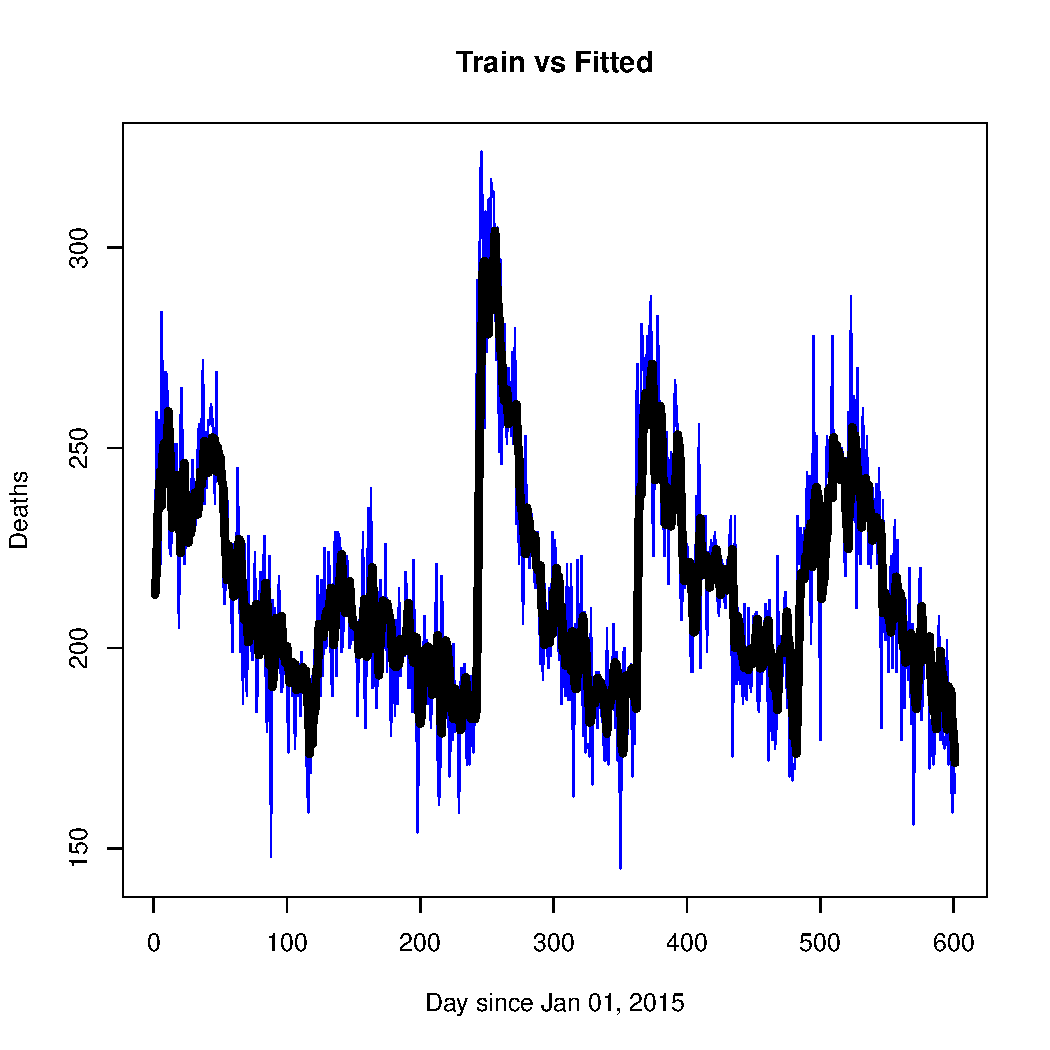
\includegraphics[width=\textwidth]{../images/fit.pdf}
	\end{subfigure}
	\begin{subfigure}[b]{0.49\textwidth}
	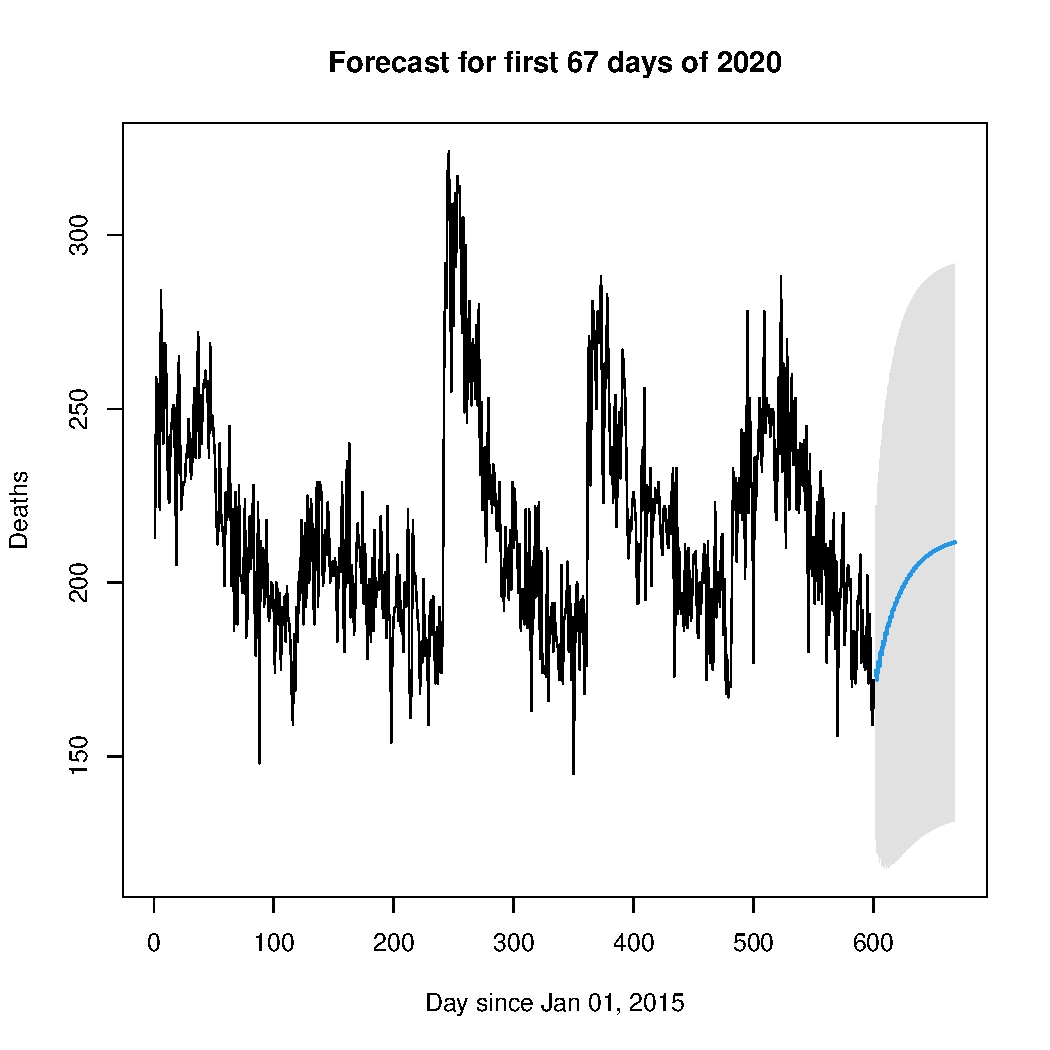
\includegraphics[width=\textwidth]{../images/forecast.pdf}
	\end{subfigure}	
	\caption{Fit of the $ARMA(3,2)$ model and forecast for 67 points.}
	\label{fig:fit_for}
\end{figure}

%The analysis has been based on the models of time series ARIMA for whose identification has been followed the Box and Jenkins procedure based on three steps: 

\section{Covid-19 deaths estimate}

Given the best model, obtained as described in the previous Section, we applied it to the 2020 data. In particular, using $99\%$ confidence intervals, we forecast the first 3 months of 2020, up to March, 27. We decided to stop at this date, and to not utilize later measures, because, according to \textbf{ISTAT} itself, they might be underestimated: the government bureau  that records deceased people could have been overwhelmed during this crisis, resulting in longer times before system updates. 

Using the forecast values as our prediction for the ``standard" deaths in 2020, we subtracted them, for each day, to the recorded values in 2020. In Figure \ref{fig:lomb_clean} we show the result of such comparison: as expected, for the first 2 months, there is no statistical significance in this data, i.e. the value $0$ is inside the confidence interval; while, starting from the first days of March, the sharp increase in deceased is still present and has a statistical significance. Indeed, even with quite large uncertainties ($\pm 80$ deaths per day), we estimate a very large amount of covid-19 related deaths.

This result is consistent with widespread knowledge about the explosion of the covid-19 pandemic in Lombardy: our spike closely corresponds with the many emergency declarations emanated by the Italian government in the first days of March. \footnote{\url{https://en.wikipedia.org/wiki/COVID-19_pandemic_in_Italy#cite_note-6}} 

\begin{figure}[h]
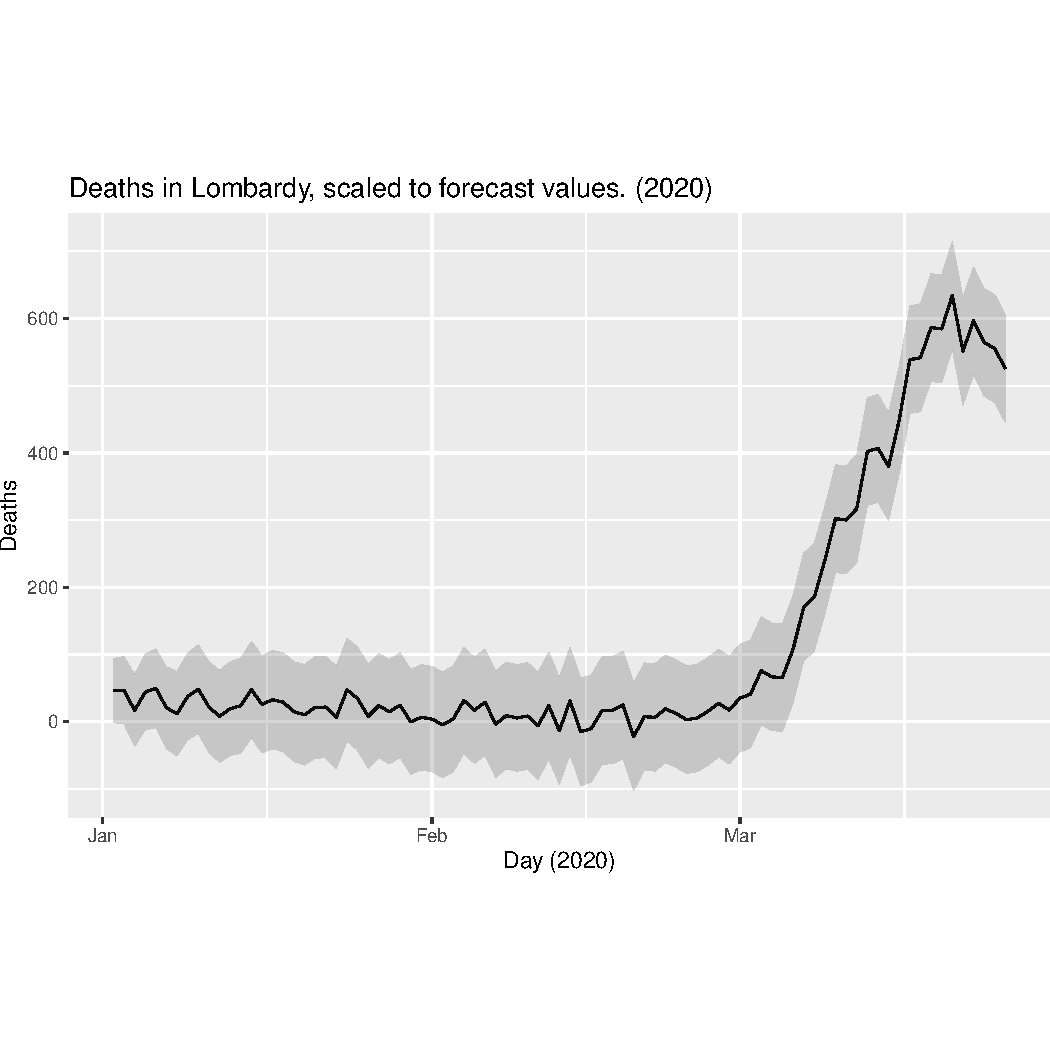
\includegraphics[width=\textwidth]{../images/lombardy_clean.pdf}
\caption{Recorded deaths scaled to the estimated values for 2020, according to our model}
\label{fig:lomb_clean}
\end{figure}

We then decided to confront it with the official count of deceased due to covid-19, as described in Section \ref{sec:descr}. We show in Figure \ref{fig:comp} this comparison, day to day. The results are astonishing: starting from March 6, the difference between the estimated death count and the reported one is statistically significant. Indeed, this graph shows how many more deaths are not reported as covid-19, but most likely are. Even with these results at hand, we cannot fully declare that all of the excess deaths are due directly to the coronavirus: some may be linked indirectly. What this means is that there could a considerable portion of these deaths that are not caused by covid-19, i.e. the person who died did not have the virus, but was not able to receive care due to multiple pandemic-related reasons, e.g. overcapacity in some hospitals.

\begin{figure}[h]
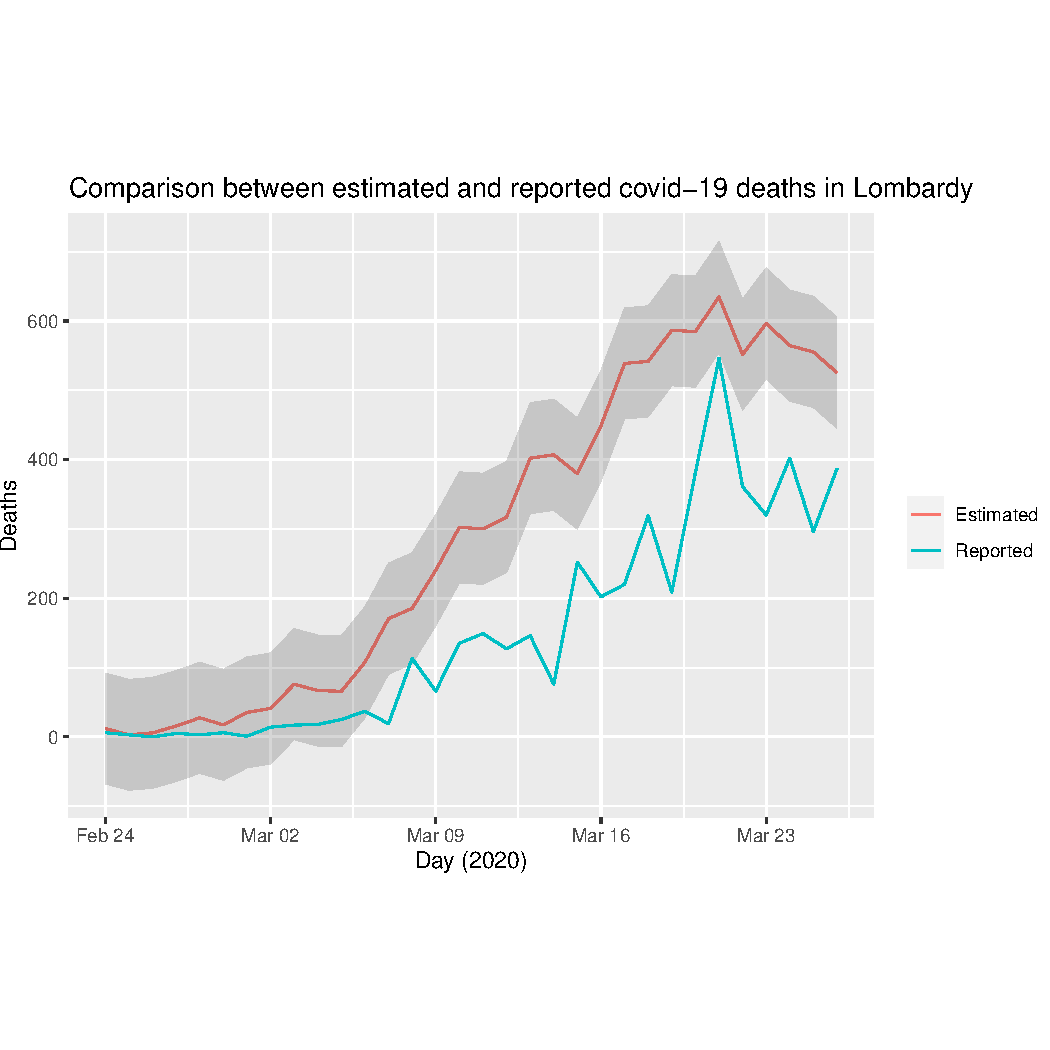
\includegraphics[width=\textwidth]{../images/confront.pdf}
\caption{Comparison between estimated covid-19 deaths and reported ones, for the period February, 24, to March, 27}
\label{fig:comp}
\end{figure}

We then decided to confront the total values for the period considered. While this was straightforward for the official deceased data, some considerations had to be done for the curve obtained with our model.

In order to calculate the cumulative values for the estimated curve, i.e. the total sum and its deviation, we had to use uncertainty propagation. Just by looking at the data, one can show that each daily deviation is approximately the same, of around  $\pm 80$ deaths per day.
 While this might be a good clue about incorrelation between each one of these, as is also the fact they come from an ARIMA model, we nevertheless decided to employ a more general method. Indeed, we approached the problem through two comparable methods:
 \begin{itemize}
 	\item Second degree Taylor approximation for the analytical formula. With this results, we did not find any difference with the incorrelated calculation.
 	\item Monte Carlo numerical evaluation, which showed a very small difference with the incorrelated case. This calculation has been carried out with a large number of simulations, and thus can be considered quite accurate.\cite{uncertainty}
 \end{itemize}
From the two previous results, one can argue that, if there is some correlation to be considered in the calculation for the cumulative deviations, it is but small and not distinguishable to a second degree approximation.

With this considerations, we found that, for the period between 2020-02-24 and 2020-03-26, we estimated the number of deceased due to covid-19 as between 8852 and  9758, with a $99\%$ confidence interval considered. 
By comparison, the total number of reported cases in the same time period is 4861, and thus there is a $182\%$ to $200\%$ increase in covid-19 related deaths compared to the official data. 

\clearpage
\section{Conclusions \& Limitations}
In conclusion, what we have found in our statistical analysis is a staggering picture of the first month of the pandemic in Northern Italy, where many more people than reported have perish because of the SARS-CoV-2 virus. Indeed, we found that, with a strong certainty, almost as double the number of people might have been killed just due to the virus, i.e. not counting the other deceased that might have happened otherwise in the same period. 

While we hope our work might inspire some bigger endeavor, we want to highlight a few limitations and problems we have faced. The first, and most important, is the \textbf{lack of data}: with this statement, we mean both the lack of historical information for the deceased in most of the year, as we had only the first 5 months; and the presence of only roughly $50\%$ of municipalities in Lombardy. The lack of months in the year certainly hindered our ability to built a more accurate model, even though we believe it might not have given too big of a difference. On the other hand, as we have described in Section \ref{sec:descr}, the lack of municipalities urged us to make stringent hypothesis in order to achieve good results. While we can safely say this did not give us a meaningless result, because, even with just half of the municipalities, we have a stark statistical difference between reported and estimated deceased, a broader picture would strengthen the final result. 

Regarding our modeling procedure, while the \textbf{ARIMA} surely did not give wrong results, the use of a simple average could have been more than sufficient for our purposes. On the other hand, we did not manage to find seasonality in the data, which, as one can probably guess by looking at the representations, might be present. Nevertheless, its effect is subtle and hardly noticeable, with differences between each year being more important than seasonal trends. With all of the months in a year at hand, one might be able to create a better and suitable model for a similar task.
s
We still hope this work can be of use for both present analysis of the pandemic and future similar scenarios. In particular, we showed how, in the early days of the rapid growth of the virus, some limitations in the testing capability and virus tracking allowed for a quite significant undercounting of the deceased.

 We conclude this short analysis with a big thanks to all of those people who are working on the front lines of this historical global pandemic, for those who put their lives at risk every day so that others can live and, at the same time, allow people like us to have readily available data.


% -- LIMITAZIONI --
% Parlare della mancanza di dati -> sia mesi che comuni
% Utilizzo della semplice media
% Problematiche del modello  -> impossibilità di trovare stagionalità
% Impossibilità di controllare aggiornamento dei dati dell'anagrafe

% -- CONCLUSIONI --
% Mancanza di preparazione a inizio epidemia
% Monito per i posteri
% Possibile approccio alla modellizzazione

\clearpage
\bibliography{./biblio_covid.bib}
\end{document}